\documentclass[
    amsfonts,
    amssymb,
    amsmath,
    reprint,
    floatfix,
    nofootinbib,
    aps,
    prl
]{revtex4-2}

\newcommand{\ManuscriptPdfTitle}{Amplitude-Robust Qubit Spectroscopy Using Echo-Root-Lorentzian Pulse Shapes}
% Encoding and language
\usepackage[T1]{fontenc}
\usepackage[utf8]{inputenc}
\usepackage[english]{babel}

% Mathematics
\usepackage{amsthm}
\usepackage{mathtools}
\usepackage{physics}

% Figures and layout
\usepackage{graphicx}
\usepackage{adjustbox}
\usepackage{placeins}
\usepackage{xcolor}

% Quotations
\usepackage{csquotes}

% Load hyperlinks last so package patches are applied consistently.
\providecommand{\ManuscriptPdfTitle}{Amplitude-Robust Qubit Spectroscopy Using Echo-Root-Lorentzian Pulse Shapes}
\usepackage[
    hidelinks,
    pdftitle={\ManuscriptPdfTitle},
    pdfauthor={Asaf A. Solonnikov and Nadav Katz}
]{hyperref}


\begin{document}

\title{Amplitude-Robust Qubit Spectroscopy Using Echo-Root-Lorentzian Pulse Shapes}

\author{Asaf A. Solonnikov and Nadav Katz}
\affiliation{The Racah Institute of Physics, The Hebrew University of Jerusalem, Israel}

\date{\today}

\begin{abstract}
We present a qubit spectroscopy method based on Lorentzian-derived drive pulses that enhances robustness against amplitude variations. Specifically, we employ a root-Lorentzian envelope with a $\pi$-phase inversion at its peak, which introduces an echo-like symmetry that cancels on-resonant Rabi oscillations while preserving the spectral response. This approach suppresses conventional power broadening and is compatible with driven-spectroscopy pulses shorter than the qubit lifetime $T_1$, a regime in which square and ordinary root-Lorentzian pulses retain amplitude-dependent coherent oscillations. Numerical simulations predict a narrow echo feature over more than three decades of peak drive. Within the independently selected experimental window of approximately $2.5$--$9~\mathrm{MHz}$, the fitted resonance center exhibits a $3~\mathrm{kHz}$ RMS displacement and a $7.5~\mathrm{kHz}$ maximum excursion, without the monotonic AC-Stark shift expected for a constant drive. We experimentally demonstrate this method on a superconducting qubit platform and observe qualitative agreement with numerical simulations, highlighting its potential for calibration-robust qubit frequency characterization as qubit lifetimes increase.
\end{abstract}


\maketitle

% Main text: keep this list in the same order as the paper.
% Spectroscopic methods span a wide range of regimes and objectives, including optical spectroscopy \cite{schawlow_infrared_1958}, nuclear magnetic (NMR) \cite{PhysRev.70.460,PhysRev.69.37}, electron spin resonance (ESR) and more. Among the most notable advances, \textit{Stimulated Emission Depletion} (STED) microscopy, introduced by Hell, surpasses the diffraction limit of light microscopy by selectively depleting fluorescence around a targeted nanoscale region, achieving resolutions on the order of tens of nanometers \cite{hell_breaking_1994,HELL199419}.  

% Parallel to these advancements, continuous efforts aim to overcome intrinsic spectral broadening mechanisms such as Doppler, Fourier (transit-time), and power broadening~\cite{PhysRevLett.104.053001,finkelstein_power_2019}. However, even in the absence of technical noise, the ultimate spectral resolution of a coherently driven two-level system is fundamentally limited by decoherence. According to the Bloch equations, the homogeneous linewidth scales inversely with the coherence time $T_2$, establishing the so-called $T_2$ limit~\cite{Zienau_1975,PhysRev.70.460}. While various schemes seek to mitigate this constraint through dynamical decoupling or engineered dissipation~\cite{PhysRevLett.122.060503,retzker_2,Cao_2025}, the connection between decoherence and spectral resolution is generally regarded as fundamental, as the same stochastic frequency fluctuations that govern dephasing also determine the resolvability of energy-level transitions.

% Experimentally, this limit is probed by weak-drive spectroscopy, in which a continuous tone is swept across the qubit transition while monitoring the excited-state population\cite{PhysRevLett.107.240501,PhysRevX.9.041041,spec123}. In this regime, the drive amplitude must remain sufficiently small to avoid power broadening, allowing the measured linewidth to approach the intrinsic decoherence-limited value.Increasing the drive strength enhances signal visibility but leads to transition saturation and a corresponding linewidth that grows approximately linearly with the drive amplitude. Conversely, excessively weak driving results in poor contrast and limits spectral resolvability. As a result, conventional spectroscopy operates within a narrow range of drive amplitudes that balances signal strength against power-induced broadening.

\begin{figure*}
    \centering
    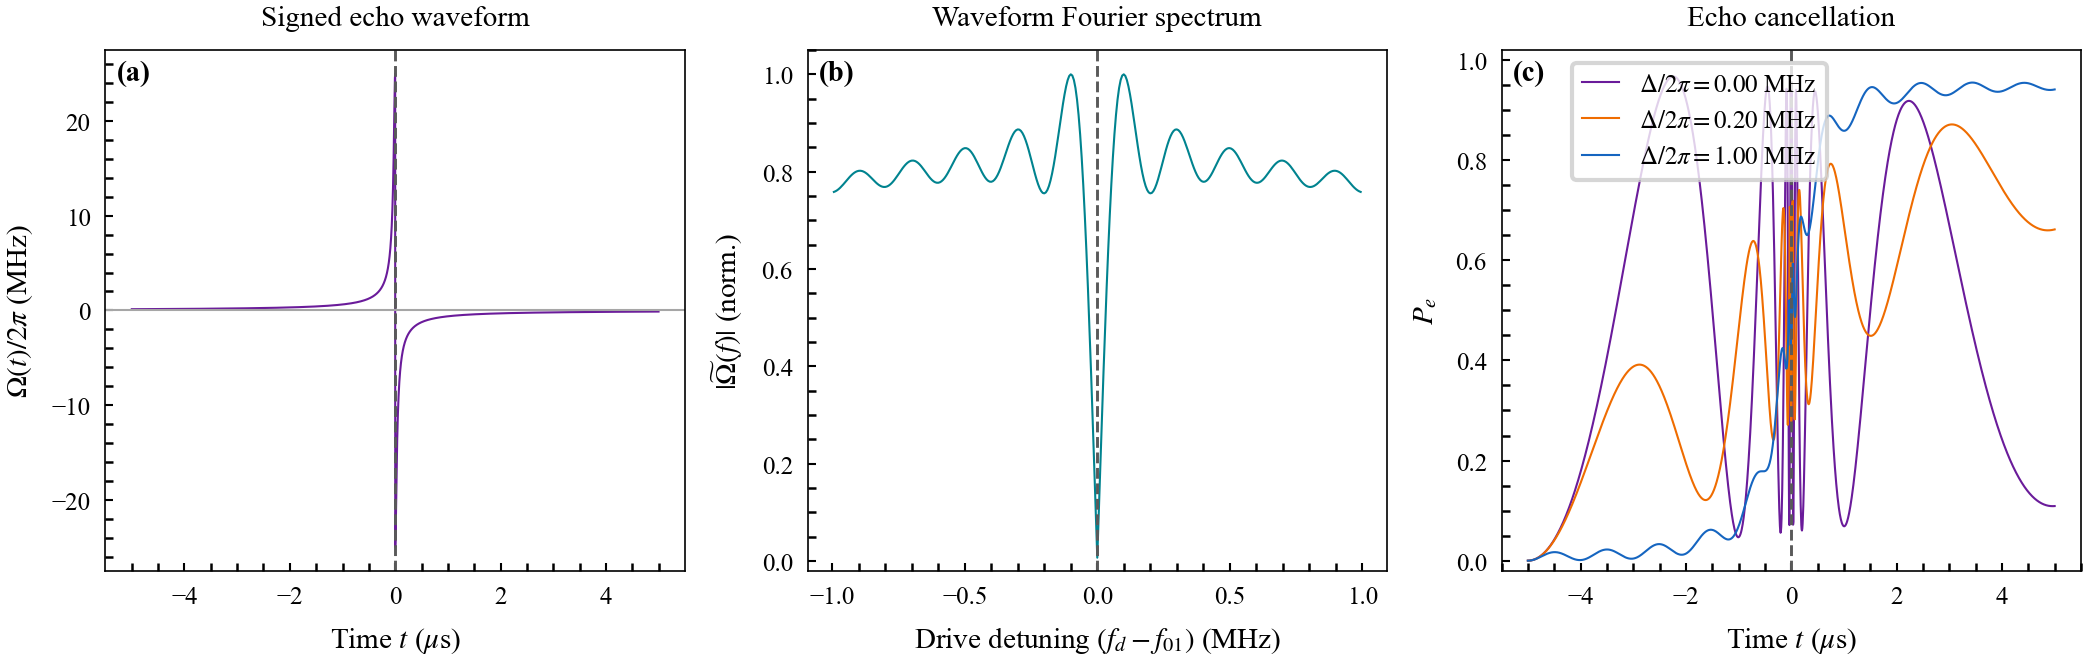
\includegraphics[width=1\linewidth]{../figures/paper/01_pulse_mechanism.png}
    \caption{
    Pulse waveform and echo-cancellation mechanism.
    (a) Signed echo-root-Lorentzian drive envelope with peak amplitude $\Omega_0/(2\pi)=15~\mathrm{MHz}$ and a $\pi$ phase inversion at the pulse midpoint.
    (b) Normalized magnitude of the waveform Fourier spectrum, showing the spectral null at zero frequency produced by the phase inversion.
    (c) Unitary two-level excited-state population during the pulse at $\Delta/(2\pi)=0$, $0.10$, and $2.00~\mathrm{MHz}$, without relaxation or dephasing. At resonance, the evolution accumulated during the first half is exactly reversed during the second half, whereas finite detuning prevents complete cancellation.}
    \label{fig:fig1}
\end{figure*}


Determining the transition frequency of a quantum system is a fundamental task
in spectroscopy, quantum metrology, and quantum sensing. The simplest setting
is a two-level system, whose energy splitting defines a spectroscopic resonance
and can encode changes in its local environment. This frequency is commonly
estimated by sweeping a coherent drive across the transition and monitoring
the resulting population response~\cite{PhysRev.70.460,PhysRev.78.695,PhysRevLett.122.060503,retzker_2}.
Such measurements underlie both the characterization of quantum devices and
the use of quantum systems as probes of external perturbations.

In direct population spectroscopy, spectral resolution and measurement
robustness are competing requirements. Conventional continuous-wave
spectroscopy generally applies a drive long enough for the population to
approach a steady state. In the weak-drive regime, decoherence produces a
homogeneous linewidth that scales as $1/T_2$, establishing the natural
coherence-limited resolution scale of the transition. Increasing the drive
strength makes the population response more pronounced, but also power broadens
the transition. Conventional high-resolution spectroscopy therefore requires
the drive amplitude to be chosen carefully, balancing a pronounced population
response against power broadening.
High-amplitude spectroscopy is further complicated when the nominal two-level
system is embedded in a multilevel spectrum. Off-resonant coupling to
neighboring transitions can produce amplitude-dependent AC-Stark shifts,
line-shape distortions, and leakage, causing the apparent resonance to move
with drive strength~\cite{PhysRevA.76.042319,motzoi_drag_2009,gambetta_analytic_2011}.






Ramsey interferometry provides a standard alternative to direct spectroscopy and, in principle, enables frequency estimation at the $T_2$ limit~\cite{PhysRev.78.695}. Other sensing protocols can surpass this probe-$T_2$ scale using inter-shot correlations, external references, dynamical decoupling, or tailored filter functions~\cite{PhysRevLett.122.060503,retzker_2,Cao_2025,gefen_clock_2016,bylander_2011,iosue_filter_2026}. Ramsey generally presupposes an approximate transition frequency and calibrated $\pi/2$ pulses for state preparation and readout, and is therefore not fully calibration independent. Achieving $T_2$-limited resolution also requires long interrogation times and sufficiently dense temporal sampling to resolve the resulting interference fringes. Finite-pulse imperfections and probe-induced frequency shifts, including unintended AC-Stark shifts during the control pulses, can nevertheless bias the extracted transition frequency~\cite{PhysRevA.98.053424,shuker_ramsey_2019}.




% In the context of superconducting circuits, circuit quantum electrodynamics (cQED) employs nonlinear harmonic oscillators—most prominently the transmon—to resolve transitions between the ground and excited states of weakly anharmonic systems. This technique, known as qubit spectroscopy, serves as a cornerstone for the calibration and characterization of superconducting quantum processors 

% Ramsey interferometry is a standard alternative to direct spectroscopy. In a typical Ramsey sequence, two $\pi/2$ pulses are separated by a free-evolution interval $\tau$, resulting in interference fringes in the excited-state population that oscillate at the detuning frequency. In practice, however, achieving $T_2$-limited spectral resolution requires both long interrogation times and sufficiently high temporal sampling to resolve the resulting oscillations. Moreover, the accuracy of Ramsey measurements is susceptible to systematic biases: asymmetries in the exponential decay envelope—arising, for example, from pulse miscalibration—can shift the perceived resonance peak in the frequency domain. Additional effects such as phase fluctuations or unintended AC-Stark shifts during the control pulses introduce further distortions, ultimately biasing the extracted frequency estimate.\cite{PhysRevA.98.053424,PhysRev.78.695,wang_coherent_2019}.

Here, we propose a spectroscopic method for probing the qubit transition frequency using an echo-root-Lorentzian drive pulse. Previous theoretical work showed that Lorentzian pulses exhibit power narrowing, complementary to the conventional power broadening observed for constant drives, as a consequence of their adiabatic properties~\cite{boradjiev_power_2013}. Power narrowing with powers-of-Lorentzian pulses was subsequently demonstrated experimentally on IBM Quantum, including the cutoff broadening introduced by truncating the pulse wings~\cite{mihov_defying_2024}. In this work, we extend this framework to longer pulse durations approaching the $T_1$ timescale and introduce a $\pi$-phase jump at the pulse peak. The resulting echo property effectively cancels the net pulse area while preserving the adiabatic properties of the drive. This phase inversion reverses the coherent phase accumulation at resonance, suppressing on-resonant excitation while maintaining an off-resonant spectral response across the frequency domain, and thus making resonance distinguishable.

\begin{figure*}[t]
    \centering
    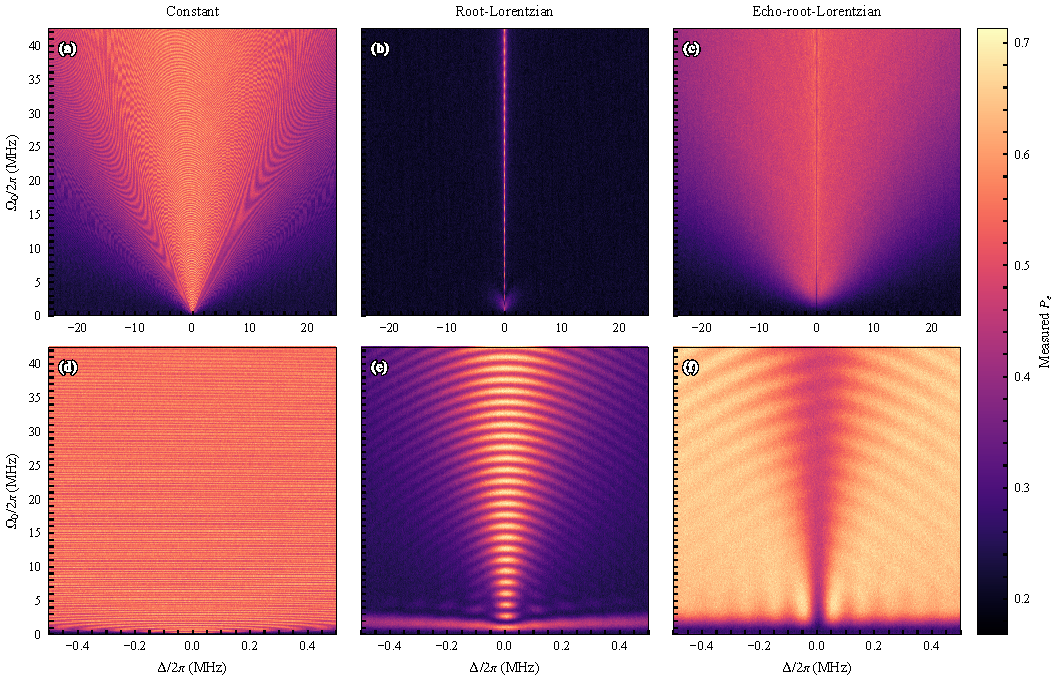
\includegraphics[width=0.92\textwidth]{../figures/paper/02_central_spectroscopy.pdf}
    \caption{
Experimental q1 spectroscopy maps for $20~\mu\mathrm{s}$ pulses.  The color
scale is the state-discriminated, measured excited-state population $P_e$.
The upper row shows the broad $100~\mathrm{MHz}$ domain ($-50$ to
$+50~\mathrm{MHz}$) with $0.5~\mathrm{MHz}$ spacing; the lower row shows the
narrow $1~\mathrm{MHz}$ domain ($-0.5$ to $+0.5~\mathrm{MHz}$) with
$5~\mathrm{kHz}$ spacing.  From left to right, the columns show a nearly
constant-envelope echo implemented as a root-Lorentzian with a
midpoint phase inversion, an ordinary root-Lorentzian with $c=0.005$, and an
echo-root-Lorentzian with $c=0.005$.  All broad maps and the narrow
constant-envelope map contain 200 shots per point.  The narrow ordinary-pulse
run contains 216 completed averages per point despite requesting 1000, while
the narrow echo-root-Lorentzian run contains all 1000.  All panels use
the same 200-point calibrated peak-Rabi grid, extending from zero to
approximately $25.1~\mathrm{MHz}$, and the same probability scale.  Active
reset and state-discriminated readout are used throughout.
The white dashed line denotes the programmed zero detuning.
    }
    \label{fig:robust-echo-spectroscopy}
\end{figure*}

\begin{figure}[t]
    \centering
    
\includegraphics[width=\columnwidth]{%
        ../figures/paper/03_lorentzian_echo_slices.pdf}
    \caption{Experimental and simulated spectra.
    (a)--(f) Final excited-state probability $P_e$ versus detuning for
    $20~\mu\mathrm{s}$ root-Lorentzian (left) and echo-root-Lorentzian (right)
    pulses with $c=0.005$.  From top to bottom,
    $\Omega_0/2\pi=3$, $20$, and $40~\mathrm{MHz}$. Continuous lines show
    three-level simulations and markers show experiment. A common global
    population offset and small gain adjustment are applied to the measured
    traces for comparison. Residual baseline mismatches remain, but the
    spectral profiles otherwise agree closely. At high drive, the echo
    response shows a line-shape discrepancy and a deeper experimental
    resonance dip, providing a stronger signal for resonance detection.
    Partial refocusing of slowly varying, non-Markovian noise by the echo
    is a possible explanation for the enhanced dip contrast relative to the
    Markovian model, consistent with noise suppression in rotary-echo
    experiments~\cite{gustavsson_rotary_echo_2012}.
    }
    \label{fig:simulation-results}
\end{figure}


We define the echo-root-Lorentzian drive from the order-$n$ generalized
Lorentzian envelope as
\begin{align}
L^{(n)}(t)
&= \frac{1}{\left[1+\left(\frac{t}{\tau}\right)^2\right]^n},
\\
L^{(1/2)}_{\mathrm{echo}}(t)
&:= L^{(1/2)}(t)\,\mathrm{sgn}(t).
\label{eq:Ln}
\end{align}
where $\tau$ sets the characteristic pulse duration and $n$ controls the
algebraic decay of the wings.

For the untruncated, plain generalized Lorentzian with $n>1/2$, the boundary of
adiabatic following provides an estimate of the characteristic spectral width.
Applying the usual adiabatic condition to this envelope gives~\cite{boradjiev_power_2013}
\begin{equation}
\Delta_b\tau
\propto
(\Omega_0 \tau)^{-\frac{1}{2n-1}},
\label{eq:lorentzian_adiabatic}
\end{equation}
where $\Delta_b$ is the angular detuning at which adiabatic following ceases
and $\Omega_0$ is the peak angular Rabi frequency.  Because the exponent is
negative, this characteristic detuning decreases as the drive strength
increases, producing power narrowing rather than conventional power broadening.
The exponent grows without bound as $n\to1/2^+$, so within its domain this
asymptotic result predicts the steepest narrowing trend at the root-Lorentzian
boundary.  At $n=1/2$, finite truncation, decoherence, and the echo phase
inversion regularize the response, and the FWHM $\Gamma_f$ used below is
therefore obtained from the complete experimental spectrum.  This
interpretation is consistent
with the power narrowing and cutoff broadening observed for powers of
Lorentzian pulses by Mihov and Vitanov~\cite{mihov_defying_2024}.  In contrast,
a square pulse exhibits conventional power broadening, with
$\Gamma_\omega\propto\Omega_0$ at large drive.  The derivation and the marginal
$n=1/2$ limit are detailed in the Supplemental Material~\cite{SupplementalMaterial}.

Spectroscopy results obtained using the echo-root-Lorentzian pulse, together
with standard square and root-Lorentzian pulses for comparison, are shown in
Fig.~\ref{fig:fig2}.  Independent measurements on qubit \CoherenceQubit{} on
\CoherenceDate{} give
$T_1=\MeasuredTOne~\mu\mathrm{s}$ and a Ramsey time
$T_2^*=\MeasuredTTwoStar~\mu\mathrm{s}$ (Supplemental Table~S1).  No
Hahn-echo decay was acquired for this data set, so the Letter does not assign
the Ramsey result to a measured Hahn-echo $T_2$.  For a conservative
measurement-linked transverse reference, we set
$T_{2,\mathrm{eff}}=T_2^*=\EffectiveTTwo~\mu\mathrm{s}$, corresponding to
$1/(\pi T_{2,\mathrm{eff}})=\EffectiveCoherenceFwhm~\mathrm{kHz}$.  The guide
lines in the cached spectroscopy panels instead reflect the historical
simulation inputs documented in Supplemental Table~S1 and are not independent
Hahn-echo evidence.

Square pulses exhibit pronounced power broadening even at low drive
amplitudes compared to Lorentzian-type pulses, with substantial linewidth
expansion observed over three orders of magnitude in amplitude.  In contrast, the root-Lorentzian pulse displays the characteristic power-narrowing behavior and maintains a narrow linewidth. However, for pulse durations comparable to the qubit lifetime $T_1$, coherent oscillations arise for both square and root-Lorentzian pulses,
resulting in amplitude-dependent linewidth variations that hinder precise
spectral extraction.

Introducing a $\pi$ phase inversion at the peak of the root-Lorentzian envelope partitions the drive into two sequential segments of opposite phase, such that the corresponding forward and backward evolutions cancel exactly at zero detuning. This echo-like structure suppresses resonant Rabi oscillations while preserving the off-resonant spectral response, producing a sharp depletion feature centered at the qubit transition frequency. In the frequency domain (Fig.~\ref{fig:fig1}), this manifests as a splitting of the spectral response accompanied by a null at resonance, rendering the measured linewidth largely insensitive to drive amplitude. This mechanism can be viewed as a Loschmidt-echo-like evolution, in which reversibility is achieved only on resonance, while detuning or decoherence breaks the cancellation and restores excitation~\cite{Gorin_2006,PhysRevA.30.1610}. Combined with the adiabatic following ensured by the Lorentzian envelope, this interference effect suppresses both power broadening and coherent Rabi oscillations, enabling narrow spectroscopy over a broad range of drive strengths and with pulse durations substantially shorter than those required by standard spectroscopy or Ramsey interferometry.

Fig.~\ref{fig:fig3} shows a numerical simulation of the qubit state evolution during the spectroscopy echo-root-Lorentzian sequence. At resonance, where the adiabatic condition breaks down, coherent Rabi oscillations are induced by the drive. However, due to the $\pi$ phase inversion at the pulse maximum, the subsequent segment of the drive reverses the accumulated evolution, resulting in a symmetric cancellation that returns the qubit close to the ground state, limited by relaxation. Measurement-linked calculations use $T_1=\MeasuredTOne~\mu\mathrm{s}$ and $T_{2,\mathrm{eff}}=\EffectiveTTwo~\mu\mathrm{s}$. The archived curve in this figure predates that coherence run and used the historical parameters listed in Supplemental Table~S1; it has not been relabeled as a simulation of the measured qubit.

For detuned drives, the system remains in the adiabatic regime throughout most of the pulse duration and undergoes excitation only in the vicinity of the pulse peak, where the phase inversion occurs. In this case, the evolution does not cancel and results in a net population transfer followed by relaxation. As a consequence, different detunings produce distinguishable final states, forming the basis of the spectroscopic response.

% Introducing a sign inversion in the root-Lorentzian envelope produces
% an effective $\pi$ phase shift in the drive, leading to a splitting of the
% carrier frequency in the spectral domain. The resulting Fourier spectrum is approximately flat in the vicinity of the qubit transition while exhibiting a null at resonance (see Fig.. This spectral structure implies that, when scanning the drive frequency, the measurement effectively probes a depletion response: excitation is suppressed at resonance and enhanced off-resonantly, producing a spectroscopic “shadow” centered at the transition frequency. In this sense, the qubit response is inferred from the absence of excitation rather than its presence.

\begin{figure}
    \centering
    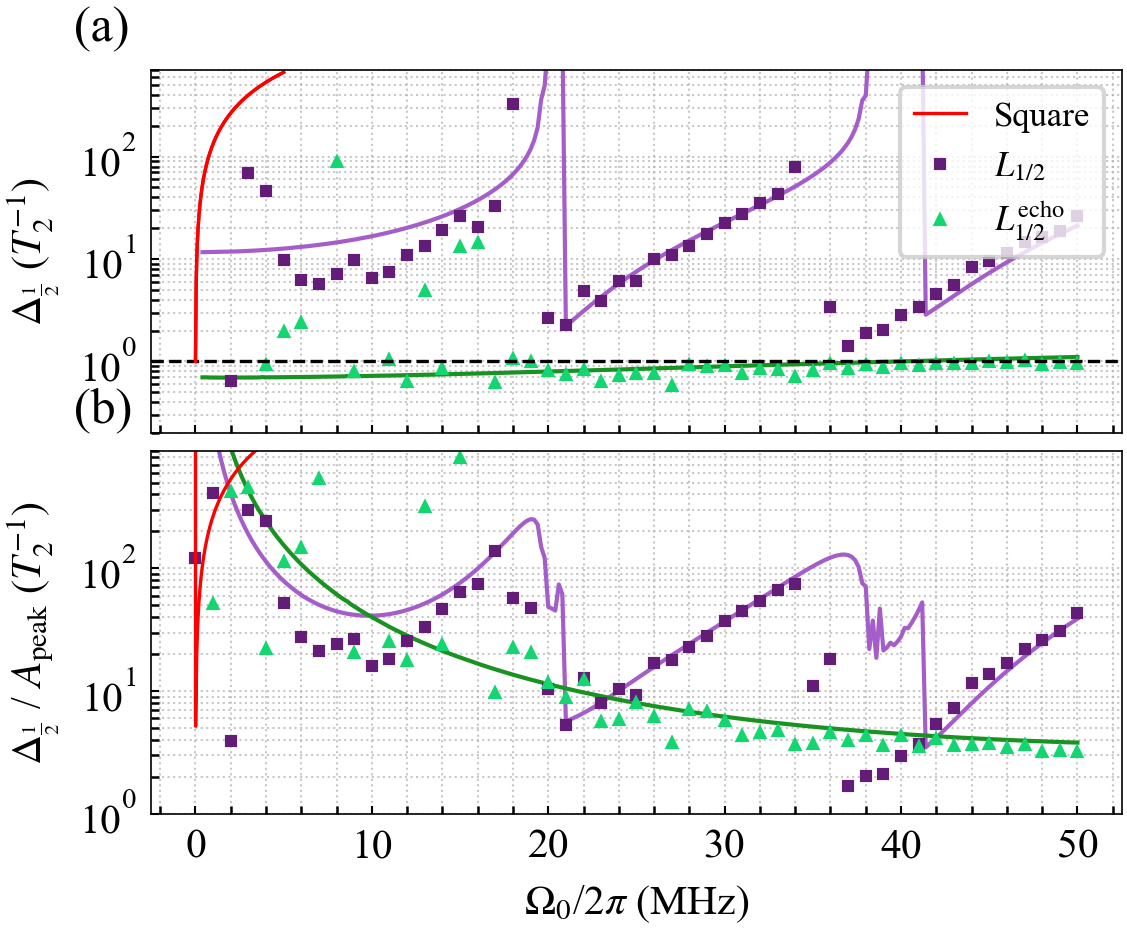
\includegraphics[width=1\linewidth]{figures/fwhm_vs_rabi_prl.png}
    \caption{
    Comparison of spectroscopic linewidth obtained using a constant (square), Lorentzian $L^{(1/2)}$, and echo-Lorentzian $L_{\text{echo}}^{(1/2)} $ drive as a function of peak Rabi frequency $\Omega_0$.
    (a) Measured full width at half maximum (FWHM) $\Delta_{1/2}$ of the qubit spectral response, normalized to the historical model-coherence scale, together with numerical simulations. Solid lines denote simulation results, while markers represent experimental data. The constant drive (red) exhibits conventional power broadening $\Delta_{1/2}\propto\Omega_0$, whereas the Lorentzian (green) and echo-Lorentzian (purple) pulses display power narrowing due to adiabatic following.
    (b) Linewidth-to-signal ratio $\Delta_{1/2}/A_{\text{peak}}$, highlighting the improved resolution--signal trade-off enabled by the echo-Lorentzian protocol at increasing drive amplitude.
    }

    \label{fig:fig4}
\end{figure}

% This mechanism is conceptually analogous to the principle underlying STED microscopy, in which a doughnut-shaped depletion beam suppresses fluorescence everywhere except at a nanoscale central node where the intensity vanishes. By scanning this engineered intensity null across the sample, fluorescence is confined to a sub-diffraction region, enabling spatial resolution beyond the diffraction limit.

% Moreover, this phase-inverted variant structure closely resembles a Loschmidt-echo–type protocol, which quantifies the reversibility of quantum dynamics under perturbations \cite{Gorin_2006,PhysRevA.30.1610}. The echo signal is defined as
% \begin{equation}
% M(t) = \left| \langle \psi_0 | e^{-i H_2 t} e^{-i H_1 t} | \psi_0 \rangle \right|^2,
% \end{equation}

% where  $H_1$  and $H_2$ denote the forward and backward Hamiltonians, respectively. Perfect time reversal ($H_2 = H_1$) yields $M(t) = 1$, while deviations—arising from detuning or noise—lead to a decay governed by decoherence processes. In our implementation, $H_1$ and $H_2$ correspond to two sequential drive segments of opposite phase, such that full reversibility is achieved only at zero detuning.
  


% Second, the echo property, implemented via a $\pi$ phase inversion at the peak of the pulse, acts as a coherent refocusing mechanism. Whereas a standard Lorentzian pulse ultimately suffers from power broadening with increasing drive strength, the phase jump reverses the accumulated phase at resonance and splits the spectral response. As a result, a destructive interference condition emerges at the carrier frequency: only at zero detuning does the forward and backward evolution cancel exactly, giving rise to a sharp and amplitude-robust null—a spectroscopic dark state. 

% The effectiveness of the echo-type Lorentzian pulse arises from two complementary mechanisms. First, the adiabatic nature of the Lorentzian envelope ensures that over a broad range of drive amplitudes the qubit state follows the instantaneous dressed eigenstate of the driven Hamiltonian. In contrast to square pulses—which introduce abrupt non-adiabatic transitions and induce oscillatory Rabi dynamics—the smooth Lorentzian profile suppresses spectral leakage and mitigates the sidebands typically associated with high-power drives.

In Fig.~\ref{fig:fig4}, we plot the extracted spectroscopic linewidth obtained from Gaussian fits to the measured response. Although the spectral lineshape of a driven two-level system is often expected to follow a Lorentzian profile, the interference-based structure of the present protocol results in a more complex response. In this regime, Gaussian fitting provides a robust and consistent estimate of the linewidth while yielding values comparable to those obtained from Lorentzian fits within our resolution requirements.

We compare the experimentally acquired linewidth extracted from two-dimensional frequency–amplitude sweeps with archived numerical simulations of an effective two-level system. The square (red), Lorentzian (green), and echo-Lorentzian (purple) drives are shown, where solid lines denote simulation results and markers represent experimental data. Because the archived curves use the historical coherence inputs in Supplemental Table~S1 rather than the later measured values, the overlay is interpreted qualitatively. For the square pulse, only simulated results are displayed. We plot both the linewidth $\Delta_{1/2}$ and the linewidth-to-signal ratio $\Delta_{1/2}/A_{\mathrm{peak}}$ to quantify the resolution–signal trade-off.

To suppress residual power broadening at large drive amplitudes, the pulse envelope must satisfy requirements on its cutoff behavior. Truncation introduces nonanalytic boundary behavior and a residual cutoff-broadening contribution that scales with the instantaneous amplitude at the cutoff point, denoted $\Omega_c$~\cite{boradjiev_qubit_2013,mihov_defying_2024,mihov_qubit_2024}. In the model, the condition $T_2^{-1}\leq\Delta_{\frac{1}{2}}$ constrains the maximum allowable cutoff amplitude to $\Omega_c<T_2^{-1}$. Empirically, we find that a relative cutoff below $10^{-3}$ suppresses excess cutoff broadening even under strong driving conditions; see the Supplemental Material for the cutoff analysis and high-amplitude measurements~\cite{SupplementalMaterial}.

% An echo-type sequence applied to the root pulse partially mitigates decoherence effects but remains limited by pronounced amplitude-dependent broadening. Conversely, the Lorentzian echo variant demonstrates an amplitude-independent linewidth spanning over three orders of magnitude in drive strength, evidencing remarkable robustness against amplitude-induced dephasing. This insensitivity arises from the adiabatic evolution and the symmetric frequency-splitting intrinsic to the pulse design. The primary limitation lies in the floating offset and amplitude-dependent baseline, resulting in reduced contrast compared to conventional square and Lorentzian drives.



To identify the useful operating regime, we examine the linewidth and contrast
of the echo response as functions of pulse duration and drive amplitude.  We
choose pulse durations shorter than $T_1$, but long enough that Fourier
broadening does not dominate.  The duration-dependent linewidth, contrast,
and contrast-weighted resolution are reported in the Supplemental
Material~\cite{SupplementalMaterial}.

A second design constraint is the cutoff of the formally infinite-support
pulse envelope.  Truncation introduces a residual endpoint drive
$\Omega_c=c\Omega_0$ and a corresponding cutoff-broadening
contribution~\cite{boradjiev_qubit_2013,mihov_defying_2024,mihov_qubit_2024}.
The relevant weak-saturation condition is
$s_c=\Omega_c^2T_1T_2\ll1$, or
$\Omega_c\ll1/\sqrt{T_1T_2}$; the inequality therefore points toward
\emph{smaller}, not larger, endpoint amplitudes.  The relative cutoff $c$
cannot be specified independently of $\Omega_0$, $T_1$, and $T_2$, giving a
three-dimensional design space of pulse duration, drive amplitude, and cutoff
level.  The corresponding cutoff--amplitude measurements and their
resolution--signal analysis are reported in the Supplemental
Material~\cite{SupplementalMaterial}.

Beyond linewidth and contrast, amplitude robustness requires that increasing
the drive not displace the inferred resonance center.  At large amplitudes,
multilevel AC-Stark shifts and finite-pulse interference become important; we
therefore examine the center stability in an additional q6 measurement
over a calibrated nominal Rabi-frequency range of $10$--$60~\mathrm{MHz}$.

\begin{figure}[t]
    \centering
    
\includegraphics[width=\columnwidth]{%
        ../figures/paper/04_main_ac_stark_correction_maps.pdf}
    \caption{Measured q6 echo-root-Lorentzian spectroscopy for (a) $\beta=0$
    and (b) $\beta=-0.22$, with $L=50~\mu\mathrm{s}$ and cutoff $c=0.00075$.
    White curves trace the fitted resonance centers. Over the
    $10$--$60~\mathrm{MHz}$ drive range, the $\beta=-0.22$ waveform shows
    smaller amplitude-dependent fluctuations of the resonance center,
    while preserving the narrow depletion feature. This waveform combines
    a DRAG quadrature with a smoothed midpoint inversion.}
    \label{fig:ac-stark-correction-maps}
\end{figure}

\begin{figure}[t]
    \centering
    
\includegraphics[width=\columnwidth]{%
        ../figures/paper/04_main_ac_stark_shifts_square.pdf}
    \caption{Resonance-center stability and linewidth of the measured
    echo-root-Lorentzian response. (a) Measured center variations
    compared with the simulated constant-drive AC-Stark shift. The measured
    curves use the same fitted centers as Fig.~\ref{fig:ac-stark-correction-maps}
    for $\beta=0$ and $-0.22$. The inset resolves their amplitude-dependent
    fluctuations over $10$--$60~\mathrm{MHz}$: the $\beta=-0.22$ waveform
    exhibits smaller center variations. The constant-drive curve retains
    the three-level simulation with
    $\alpha/(2\pi)=\MeasuredAnharmonicity~\mathrm{MHz}$.
    (b) Gaussian-fit FWHM of the same measured spectra and the red
    constant-drive power-broadening reference, on a logarithmic scale.
    The right axis expresses linewidths in units of the paper's q1
    reference $\Gamma_{T_2}=\EffectiveCoherenceFwhm~\mathrm{kHz}$ (dotted line).
    Both measured waveforms broaden with drive, while the $\beta=0$
    response exhibits larger linewidth excursions at high amplitudes.}
    \label{fig:main-ac-stark-shifts}
\end{figure}

For comparison, the weak-drive three-level AC-Stark shift of a constant drive
is $\delta f_{01}\simeq-\left(\Omega_0/2\pi\right)^2/
[2(\alpha/2\pi)]$~\cite{PhysRevA.76.042319,schneider_multilevel_2018}.
With $\alpha/(2\pi)=\MeasuredAnharmonicity~\mathrm{MHz}$, it reaches
$5.8~\mathrm{MHz}$ at $\Omega_0/(2\pi)=50~\mathrm{MHz}$.  For the
$20~\mu\mathrm{s}$ root-Lorentzian envelope with $c=0.001$, the phase-average
shift is smaller by $\langle f^2\rangle_t=0.001570$ and reaches only
$9.1~\mathrm{kHz}$; the echo sign change does not cancel this quadratic term.
Fig.~\ref{fig:ac-stark-correction-maps} instead tests a derivative-quadrature
waveform on q6 in the September 5--6 calibration campaign. The acquisition
uses $I+iQ$ with $Q=-\beta\dot I/(2\pi\alpha_{\rm cal})$, where
$\alpha_{\rm cal}=237.95~\mathrm{MHz}$ is the signed value supplied to the
waveform generator and time is in microseconds. Both the derivative
quadrature and the midpoint smoothing change between these sequential runs;
no accumulated-phase correction is applied. The depletion feature persists
across the displayed $10$--$60~\mathrm{MHz}$ range in both maps. For display,
we subtract each run's arithmetic mean accepted fitted center over this
range, $20.85$ and $36.68~\mathrm{kHz}$ relative to the acquisition reference
for $\beta=0$ and $-0.22$, respectively. The RMS residual center motion is
$6.78$ and $2.64~\mathrm{kHz}$ about these respective means. This lower
scatter characterizes the combined smoothed-midpoint and DRAG waveform;
the comparison does not isolate the derivative-quadrature contribution.
The absence of resolved three-state readout precludes a measured
leakage-suppression claim.

Fig.~\ref{fig:main-ac-stark-shifts}(a) compares these measured center
variations with the original three-level constant-drive simulation. The
experimental curves retain the centering used in
Fig.~\ref{fig:ac-stark-correction-maps}; the simulated curve is referenced
to the bare transition and retains the q1 anharmonicity
$\alpha/(2\pi)=\MeasuredAnharmonicity~\mathrm{MHz}$ as an illustrative scale
comparison. Its megahertz-scale displacement contrasts with the kilohertz-scale
residual motion of the measured echo resonances. The inset magnifies the
$\pm16~\mathrm{kHz}$ region around the mean centers.
Panel (b) compares FWHM values extracted
from the same Gaussian dip estimator with the steady-state Bloch reference
$\Gamma=\Gamma_{T_2}\sqrt{1+\Omega^2T_1T_2}$, using the paper's q1 values
$T_1=\MeasuredTOne~\mu\mathrm{s}$ and $T_2=\EffectiveTTwo~\mu\mathrm{s}$.
The right axis uses the same q1 coherence reference, rather than a separate
q6 coherence calibration. Both measured linewidths increase with drive;
the smaller center fluctuations for $\beta=-0.22$ therefore do not imply
a uniformly narrower resonance. Numerical accumulated-phase compensation
is discussed separately in the Supplemental Material~\cite{SupplementalMaterial}.

\par
In conclusion, we have demonstrated a narrow spectroscopic depletion feature
that persists over more than three decades of peak drive. Measurements
establish its linewidth, contrast, drive-induced center motion, and
accumulated-phase compensation. The agreement between the measured spectra
and the numerical curves in Fig.~\ref{fig:simulation-results} validates the
model. Phase-inverted shaped pulses therefore provide a practical route
to high-resolution qubit spectroscopy beyond the weak-drive regime.


\input{backmatter/acknowledgements}

% The supporting sections are compiled separately from supplemental.tex.
\bibliography{references}

\end{document}
